\documentclass[a4paper, 10pt]{article}

\usepackage[default]{comfortaa}
\usepackage[utf8]{inputenc}
\usepackage[english]{babel}
\usepackage{graphicx}
\usepackage{pdflscape}
\usepackage{geometry}
\usepackage{titlesec}
\usepackage{multicol}
\usepackage{lastpage}
\usepackage{fancyhdr}
\usepackage{array}
\usepackage{multirow, hhline}
\usepackage[table]{xcolor}
\usepackage[hidelinks]{hyperref}
\usepackage{textcomp}

\setlength{\columnseprule}{1pt}
\setlength{\columnsep}{1cm}

\definecolor{lightgray}{gray}{0.85}

\setlength{\arrayrulewidth}{0.35mm}
\setlength{\tabcolsep}{10pt}
\renewcommand{\arraystretch}{1.7}

\fancypagestyle{plain}{%
\fancyhf{} % clear all header and footer fields
\cfoot{\thepage /\pageref{LastPage}}
\rfoot{\href{https://github.com/ElectricCanary/FXCoreModule}{
\includegraphics[width=5mm, height=5mm]{github}}\hspace{8pt}\href{https://www.facebook.com/ElectricCanary}{
\includegraphics[width=5mm, height=5mm]{f}}\hspace{8pt}\href{https://www.instagram.com/electricanary/}{
\includegraphics[width=5mm, height=5mm]{inst}}\hspace{12pt}\href{mailto:support@electric-canary.com}{
\includegraphics[width=5mm, height=5mm]{email}}}
\lfoot{\textcolor{black!70}{{\footnotesize\textcopyright Electric Canary - January 2021}}}
\renewcommand{\headrulewidth}{0pt}
\renewcommand{\footrulewidth}{0pt}}


\pagestyle{fancy}
\renewcommand{\headrulewidth}{0pt}
\cfoot{}
\cfoot{\thepage /\pageref{LastPage}}
\rfoot{\href{https://github.com/ElectricCanary/FXCoreModule}{
\includegraphics[width=5mm, height=5mm]{github}}\hspace{8pt}\href{https://www.facebook.com/ElectricCanary}{
\includegraphics[width=5mm, height=5mm]{f}}\hspace{8pt}\href{https://www.instagram.com/electricanary/}{
\includegraphics[width=5mm, height=5mm]{inst}}\hspace{12pt}\href{mailto:support@electric-canary.com}{
\includegraphics[width=5mm, height=5mm]{email}}}
\lfoot{\textcolor{black!70}{{\footnotesize\textcopyright Electric Canary - January 2022}}}
\rhead{\href{https://electric-canary.com/bontempo}{
\includegraphics[scale=0.22]{logo}}}
\lhead{\textbf{{\small\emph{\textcolor{black!70}{FXCore Module-Datasheet}}}}}

\titleformat*{\section}{\huge\bfseries}
\titleformat*{\subsection}{\LARGE\bfseries}
\titleformat*{\subsubsection}{\Large\bfseries}

\geometry{hmargin=2.5cm,vmargin=2.5cm}
\headheight=35pt

\begin{document}\thispagestyle{plain}
\begin{center}
\begin{Huge}
\vspace*{0.5cm}
\textbf{FXCore Module - Datasheet}
\rule {0.95\textwidth}{2pt}\\
\end{Huge}
\vspace{1cm}

\includegraphics[scale=1]{logocentre}\\
\vspace{1cm}
\end{center}

\begin{multicols}{2}
\section{Introduction}
\bigbreak
FXCore Module is an extremely compact stereo development board for the Experimental Noize FXCore DSP. It makes the FXCore breadboard friendly and easily incorporated in a project.\\

The power module assures very efficient power delivery for a very large range of input voltage. The micro-controller allows for a very easy program selection with a single potentiometer.\\

The FXCore Module opens the door to a world of powerful DSP effects with a plethora of controls.
\vfill\null
\columnbreak

\section{Features}
\bigbreak
\begin{itemize}
\item Stereo Line In \& Out
\item Onboard 5V to 3V3 Onboard Linear Regulator
\item Easy Analog Program Selection
\item Onboard Clipping LED
\item Extremely Compact Design
\item Breadboard Compatible
\item Easy Access to Tap-Tempo, Bypass \& User Outputs
\end{itemize}
\end{multicols}

\newpage
\headheight=35pt
\tableofcontents
\newpage

\section{Pin Configuration}
\label{sec:pinconfig}
\begin{center}
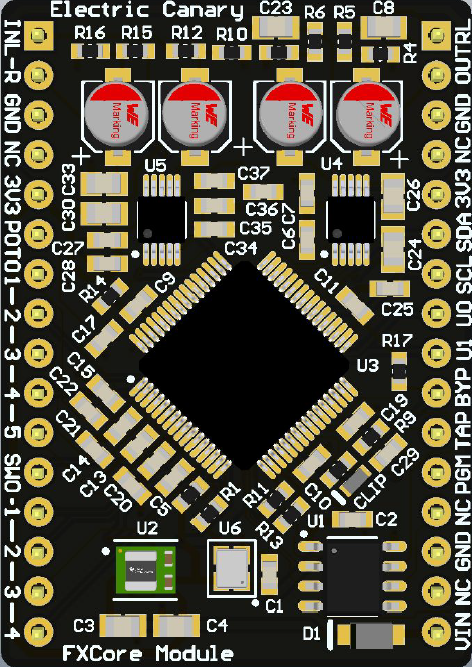
\includegraphics[scale=0.66]{FXCoreimg}\\
\begin{table}[h!]
{\rowcolors{1}{}{lightgray!50}
\begin{tabular}{|m{0.5cm}|m{4.5cm}|m{0.7cm}|m{7.5cm}|}
\hline
\rowcolor{gray} \centering \textcolor{white}{\Large\textbf{N°}} & \centering \textcolor{white}{\Large\textbf{Name}} & \centering \textcolor{white}{\Large\textbf{I/O}} & \textcolor{white}{\Large\textbf{Description}}\\
\hline
\centering 1 & \centering INL & \centering I & Left Line Audio Input\\
\hline
\centering 2 & \centering INR & \centering I & Right Line Audio Input\\
\hline
\centering 3 & \centering GND & \centering I & Ground\\
\hline
\centering 4 & \centering NC & \centering X & Not Connected\\
\hline
\centering 5 & \centering 3V3 & \centering I & +3.3V Power Input\\
\hline
\centering 6 & \centering POT0 & \centering I & Analog Input for Potentiometer 0\\
\hline
\centering 7 & \centering POT1 & \centering I & Analog Input for Potentiometer 1\\
\hline
\centering 8 & \centering POT2 & \centering I & Analog Input for Potentiometer 2\\
\hline
\centering 9 & \centering POT3 & \centering I & Analog Input for Potentiometer 3\\
\hline
\centering 10 & \centering POT4 & \centering I & Analog Input for Potentiometer 4\\
\hline
\centering 11 & \centering POT5 & \centering I & Analog Input for Potentiometer 5\\
\hline
\centering 12 & \centering SW0 & \centering I & Digital Input for Switch 0\\
\hline
\centering 13 & \centering SW1 & \centering I & Digital Input for Switch 1\\
\hline
\centering 14 & \centering SW2 & \centering I & Digital Input for Switch 2\\
\hline
\centering 15 & \centering SW3 & \centering I & Digital Input for Switch 3\\
\hline
\centering 16 & \centering SW4 & \centering I & Digital Input for Switch 4\\
\hline
\end{tabular}}
\caption{Pin Configuration}
\end{table}
\begin{table}[h!]
{\rowcolors{1}{}{lightgray!50}
\begin{tabular}{|m{0.5cm}|m{4.5cm}|m{0.7cm}|m{7.5cm}|}
\hline
\rowcolor{gray} \centering \textcolor{white}{\Large\textbf{N°}} & \centering \textcolor{white}{\Large\textbf{Name}} & \centering \textcolor{white}{\Large\textbf{I/O}} & \textcolor{white}{\Large\textbf{Description}}\\
\hline
\centering 17 & \centering VIN & \centering I & 5V Linear Regulator Input\\
\hline
\centering 18 & \centering NC & \centering X & Not Connected\\
\hline
\centering 19 & \centering GND & \centering I & Ground\\
\hline
\centering 20 & \centering NC & \centering I/O & Not Connected in Normal Operation (UPDI Pin of U1)\\
\hline
\centering 21 & \centering PGM & \centering I & Analog Input for Selecting one of the 16 Programs\\
\hline
\centering 22 & \centering TAP & \centering I & Digital Input for Tap Tempo\\
\hline
\centering 23 & \centering BYP & \centering I & Digital Input for Bypass\\
\hline
\centering 24 & \centering U1 & \centering O & Digital User 1 Output \\
\hline
\centering 25 & \centering U0 & \centering O & Digital User 0 Output\\
\hline
\centering 26 & \centering SCL & \centering I/O & Serial Clock Wire of the FXCore I2C Programming Bus\\
\hline
\centering 27 & \centering SDA & \centering I/O & Serial Data Wire of the FXCore I2C Programming Bus\\
\hline
\centering 28 & \centering 3V3 & \centering I & +3.3V Power Input\\
\hline
\centering 29 & \centering NC & \centering X & Not Connected\\
\hline
\centering 30 & \centering GND & \centering I & Ground\\
\hline
\centering 31 & \centering OUTR & \centering O & Right Line Audio Output\\
\hline
\centering 32 & \centering OUTL & \centering O & Left Line Audio Output\\
\hline
\end{tabular}}
\caption{Pin Configuration (continued)}
\end{table}
\end{center}
\newpage

\section{Absolute Maximum Ratings}
\begin{table}[h!]
\centering
{\rowcolors{1}{}{lightgray!50}
\begin{tabular}{|c|c|c|c|}
\hline
\rowcolor{gray}\textcolor{white}{\Large\textbf{Parameter}} & \textcolor{white}{\Large\textbf{Min}} & \textcolor{white}{\Large\textbf{Max}} & \textcolor{white}{\Large\textbf{Unit}}\\
\hline
Storage Temperature & -40 & +140 & °C\\
\hline
Operating Temperature & -30 & +80 & °C\\
\hline
+3.3V Voltage & -0.3 & +6 & V\\
\hline
VIn Voltage & -0.3 & +6.5 & V\\
\hline
Audio Line In Voltage & -0.7 & +7 & V\\
\hline
Audio Line In Current & -10 & +10 & mA\\
\hline
PGM Pin Voltage & -0.5 & +3.8 & V\\
\hline
PGM Pin Current & -40 & +40 & mA\\
\hline
\end{tabular}}
\caption{Absolute Maximum Ratings}
\end{table}

\section{Characteristics}
\bigbreak
\begin{table}[h!]
\centering
\begin{tabular}{|c|c|c|c|c|}
\hline
\rowcolor{gray}\textcolor{white}{\Large\textbf{Parameter}} & \textcolor{white}{\Large\textbf{Min}} &  \textcolor{white}{\Large\textbf{Typ.}} & \textcolor{white}{\Large\textbf{Max}} & \textcolor{white}{\Large\textbf{Unit}}\\
\hline
3.3V Power Supply & 3.2 & 3.3 & 3.42 & V\\
\hline
VIn Power Supply & 4 & 5 & 6 & V\\
\hline
3.3V Current & - & 155 & - & mA\\
\hline
Power Module Supply Switching Frequency & 675 & 750 & 825 & kHz\\
\hline
POT0 – POT5 source impedance & - & - & 10 & k$\Omega$\\
\hline
Input low voltage to SWO – SW4, ENABLE and TAP & GND & - & 0.66 & V\\
\hline
Input high voltage to SWO – SW4, ENABLE and TAP & 2.64 & - & 3.3 & V\\
\hline
Output low voltage to USER0 \& USER1 & 0 & - & 0.4 & V\\
\hline
Output high voltage to USER0 \& USER1 & 2.4 & - & 3.3 & V\\
\hline
Estimated FLASH endurance (Erase/Write cycles) & - & 10 000 & - & -\\
\hline
Sample rate range & 9.766 & 48 & 48.046 & kHz\\
\hline
Dynamic Range & 86 & 94 & - & dBA\\
\hline
Full Scale Input Voltage & 3.7 & 3.75 & 3.8 & Vpp\\
\hline
Full Scale Output Voltage & 2 & 2.15 & 2.3 & Vpp\\
\hline
\end{tabular}
\caption{Characteristics}
\end{table}

\begin{landscape}
\section{Typical Application Schematic}
\begin{center}
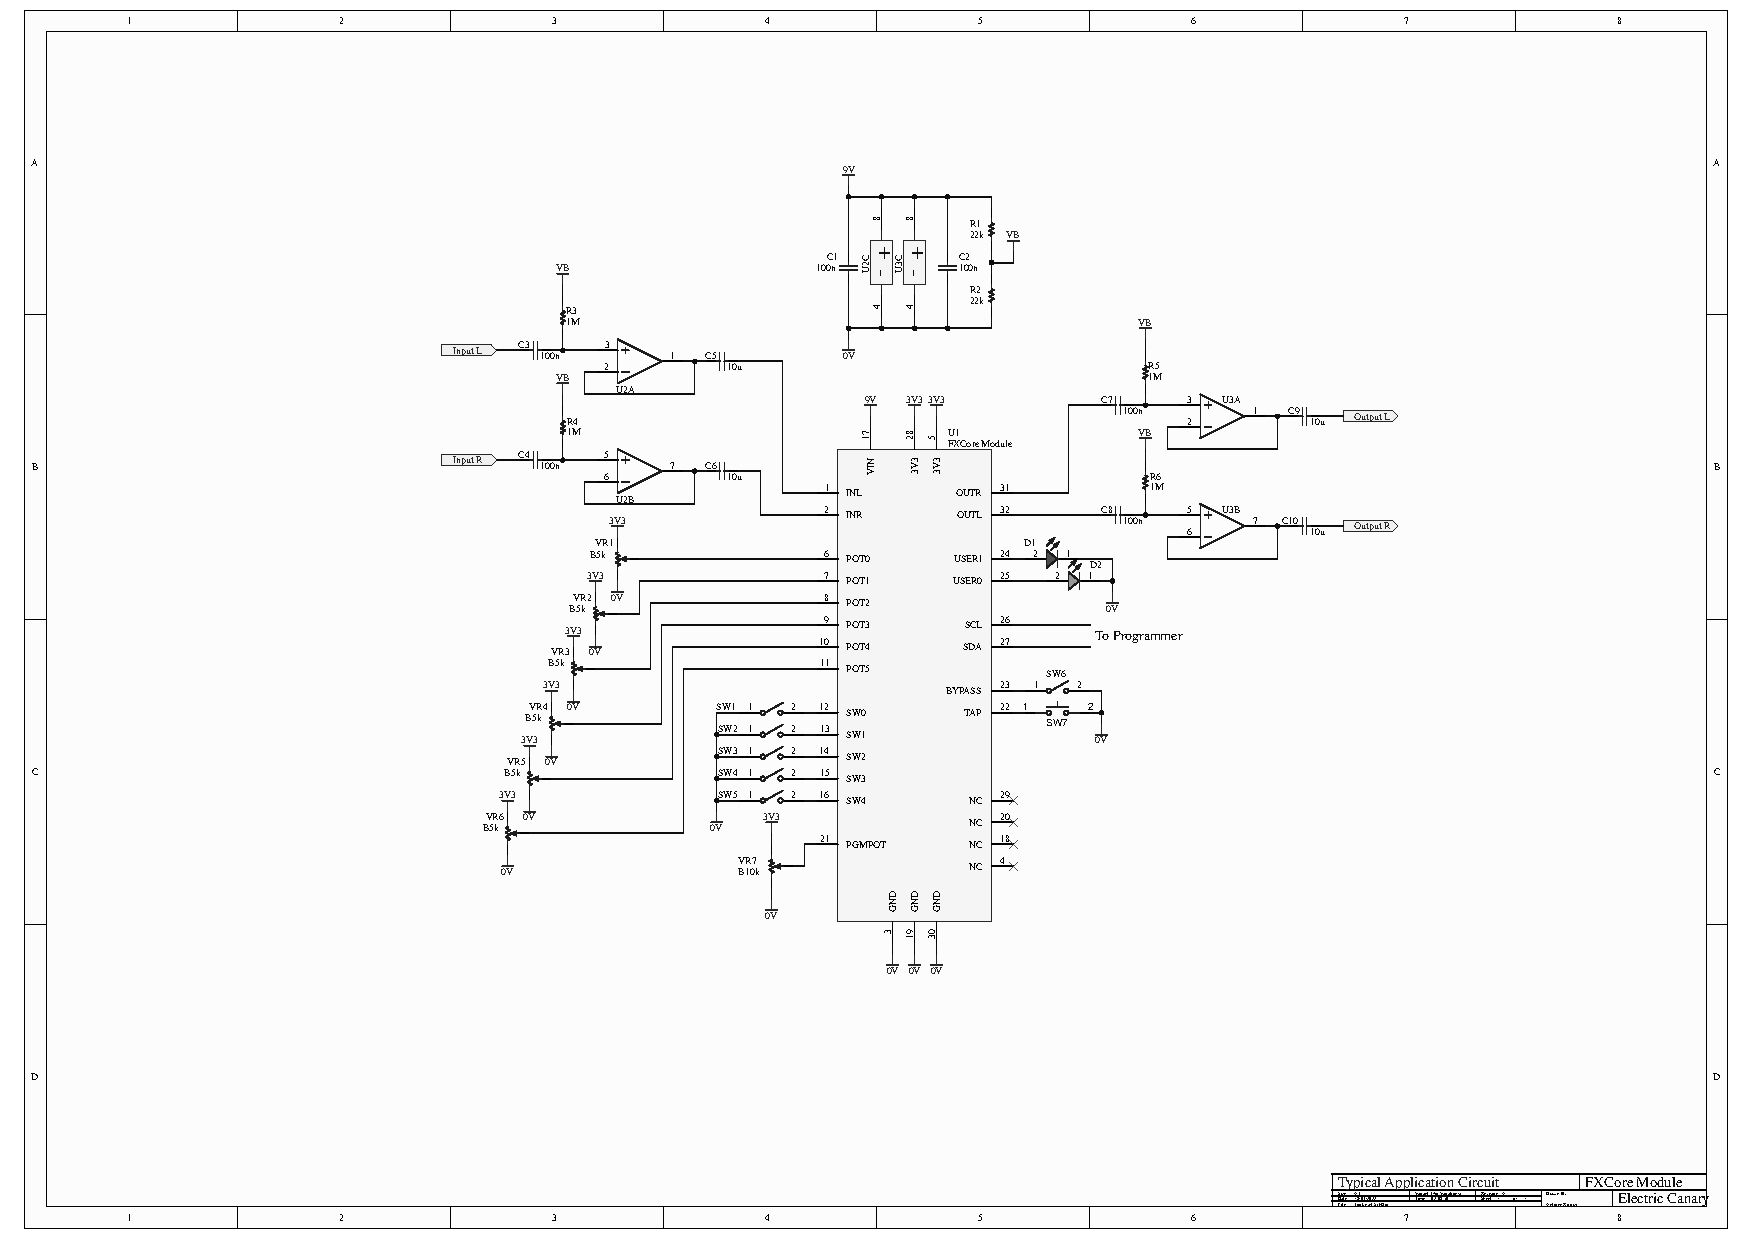
\includegraphics[scale = 0.7]{TypicalAppSch.pdf}
\end{center}
\end{landscape}
\newpage

\begin{landscape}
\section{Schematic}
\begin{center}
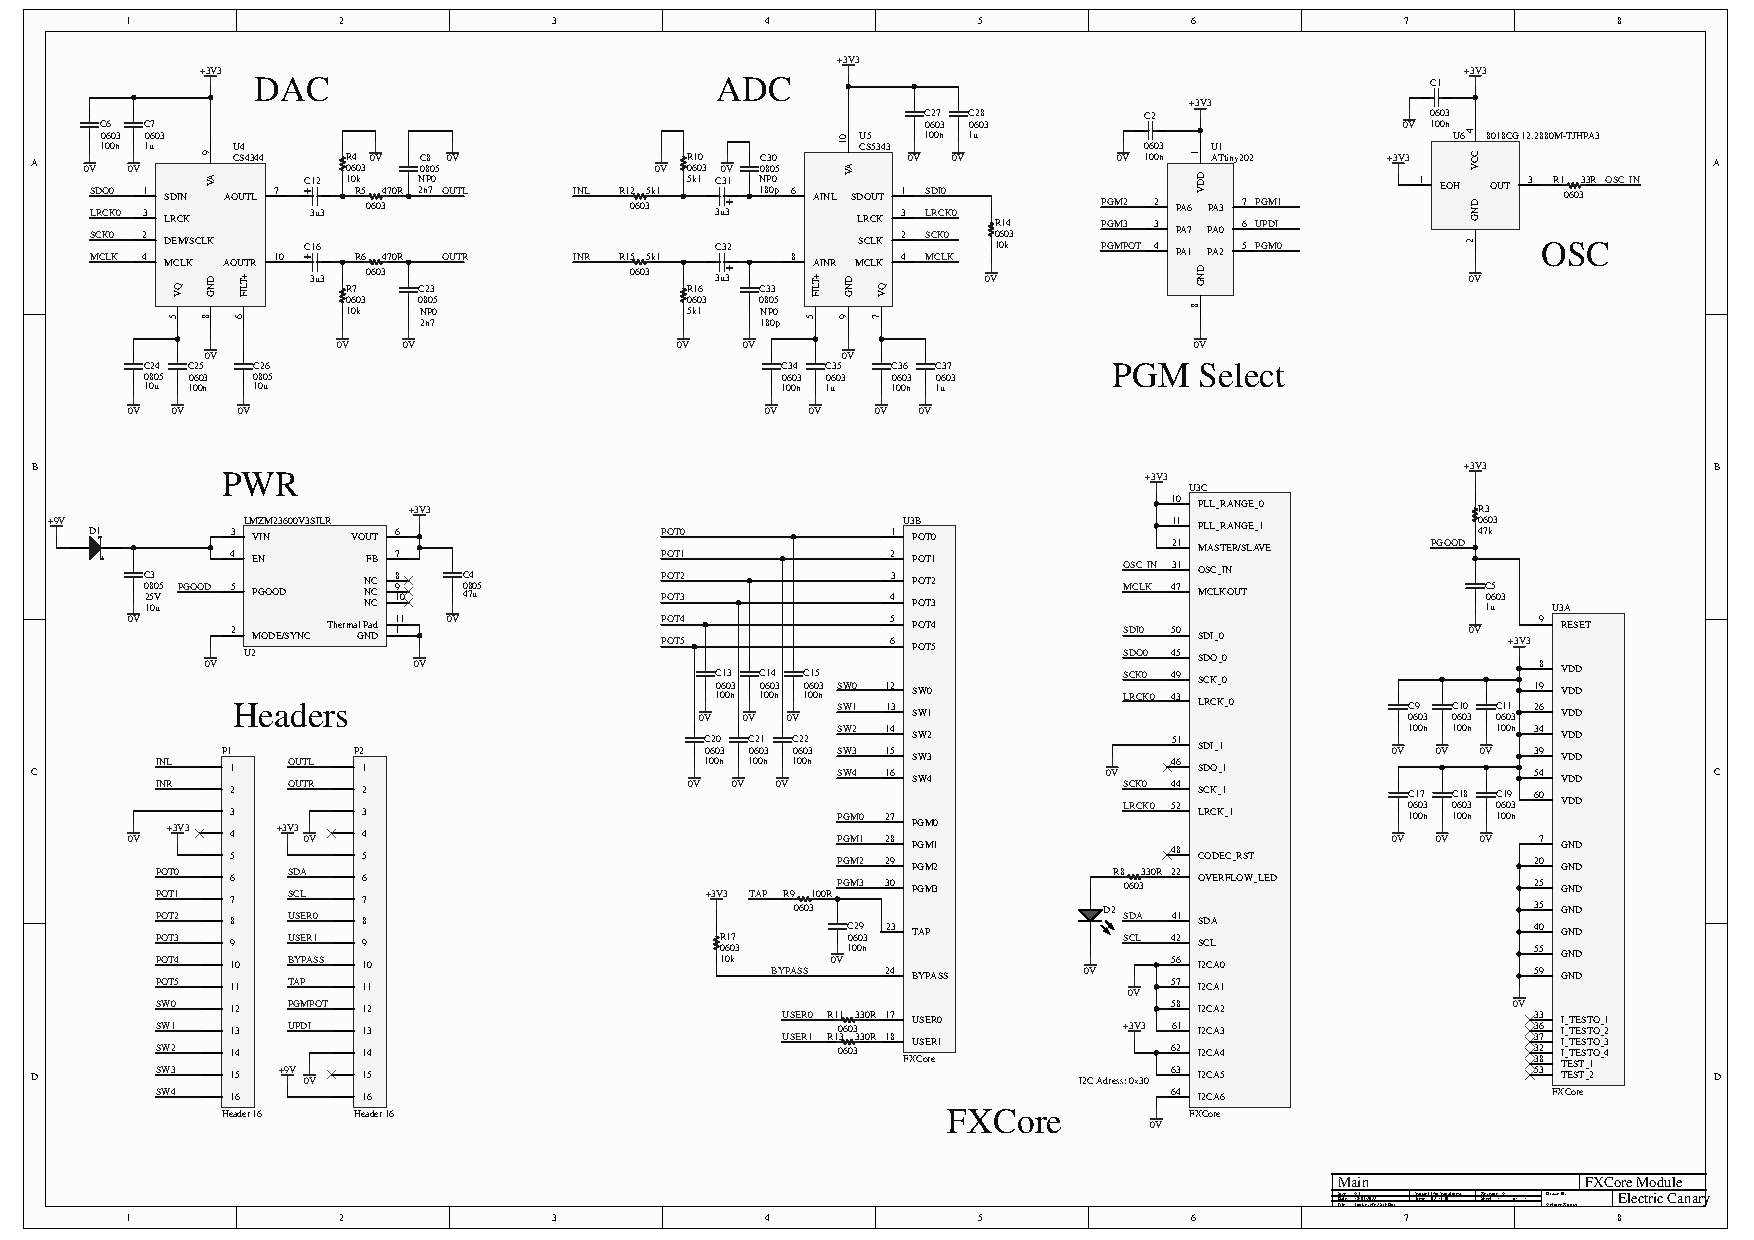
\includegraphics[scale = 0.7]{Schematic.pdf}
\end{center}
\end{landscape}
\newpage

\section{Bill of Materials}
{\rowcolors{1}{}{lightgray!50}
\begin{tabular}{|c|c|}
\hline
\rowcolor{gray}{\LARGE\textcolor{white}{\textbf{Name}}} &  {\LARGE\textcolor{white}{\textbf{Value}}}\\
\hline
R1 & 33$\Omega$\\
\hline
R3 & 47k$\Omega$ \\
\hline
R4, R7, R14, R17 & 10k$\Omega$ \\
\hline
R5, R6 & 470$\Omega$ \\
\hline
R8, R11, R13 & 330$\Omega$ \\
\hline
R9 & 100$\Omega$ \\
\hline
R10, R12, R15, R16 & 5.1k$\Omega$ \\
\hline
 &  \\
\hline
C1, C2, C6, C9, C10, C11, C13, C14, C15, C17, C18, C19, C20, C21, C22, C25, C27 & 100nF \\
\hline
C3, C24, C26 & 10$\mu$F \\
\hline
C4 & 47$\mu$F \\
\hline
C5, C7, C28, C35, C37 & 1$\mu$F \\
\hline
C8, C23 & 2.7nF \\
\hline
C12, C16, C31, C32 & 3.3$\mu$F \\
\hline
 &  \\
\hline
D1 & Schottky \\
\hline
D2 & LED \\
\hline
 &  \\
\hline
P1, P2 & 16 Pin Header \\
\hline
 &  \\
\hline
U1 & ATtiny202 \\
\hline
U2 & AP7365-33ERG-13 \\
\hline
U3 & FXCore \\
\hline
U4 & CS4344 \\
\hline
U5 & CS5343 \\
\hline
U6 & 12.288MHz Oscillator \\
\hline
\end{tabular}}
\newpage

\section{Assembly}
\begin{center}
\vfill
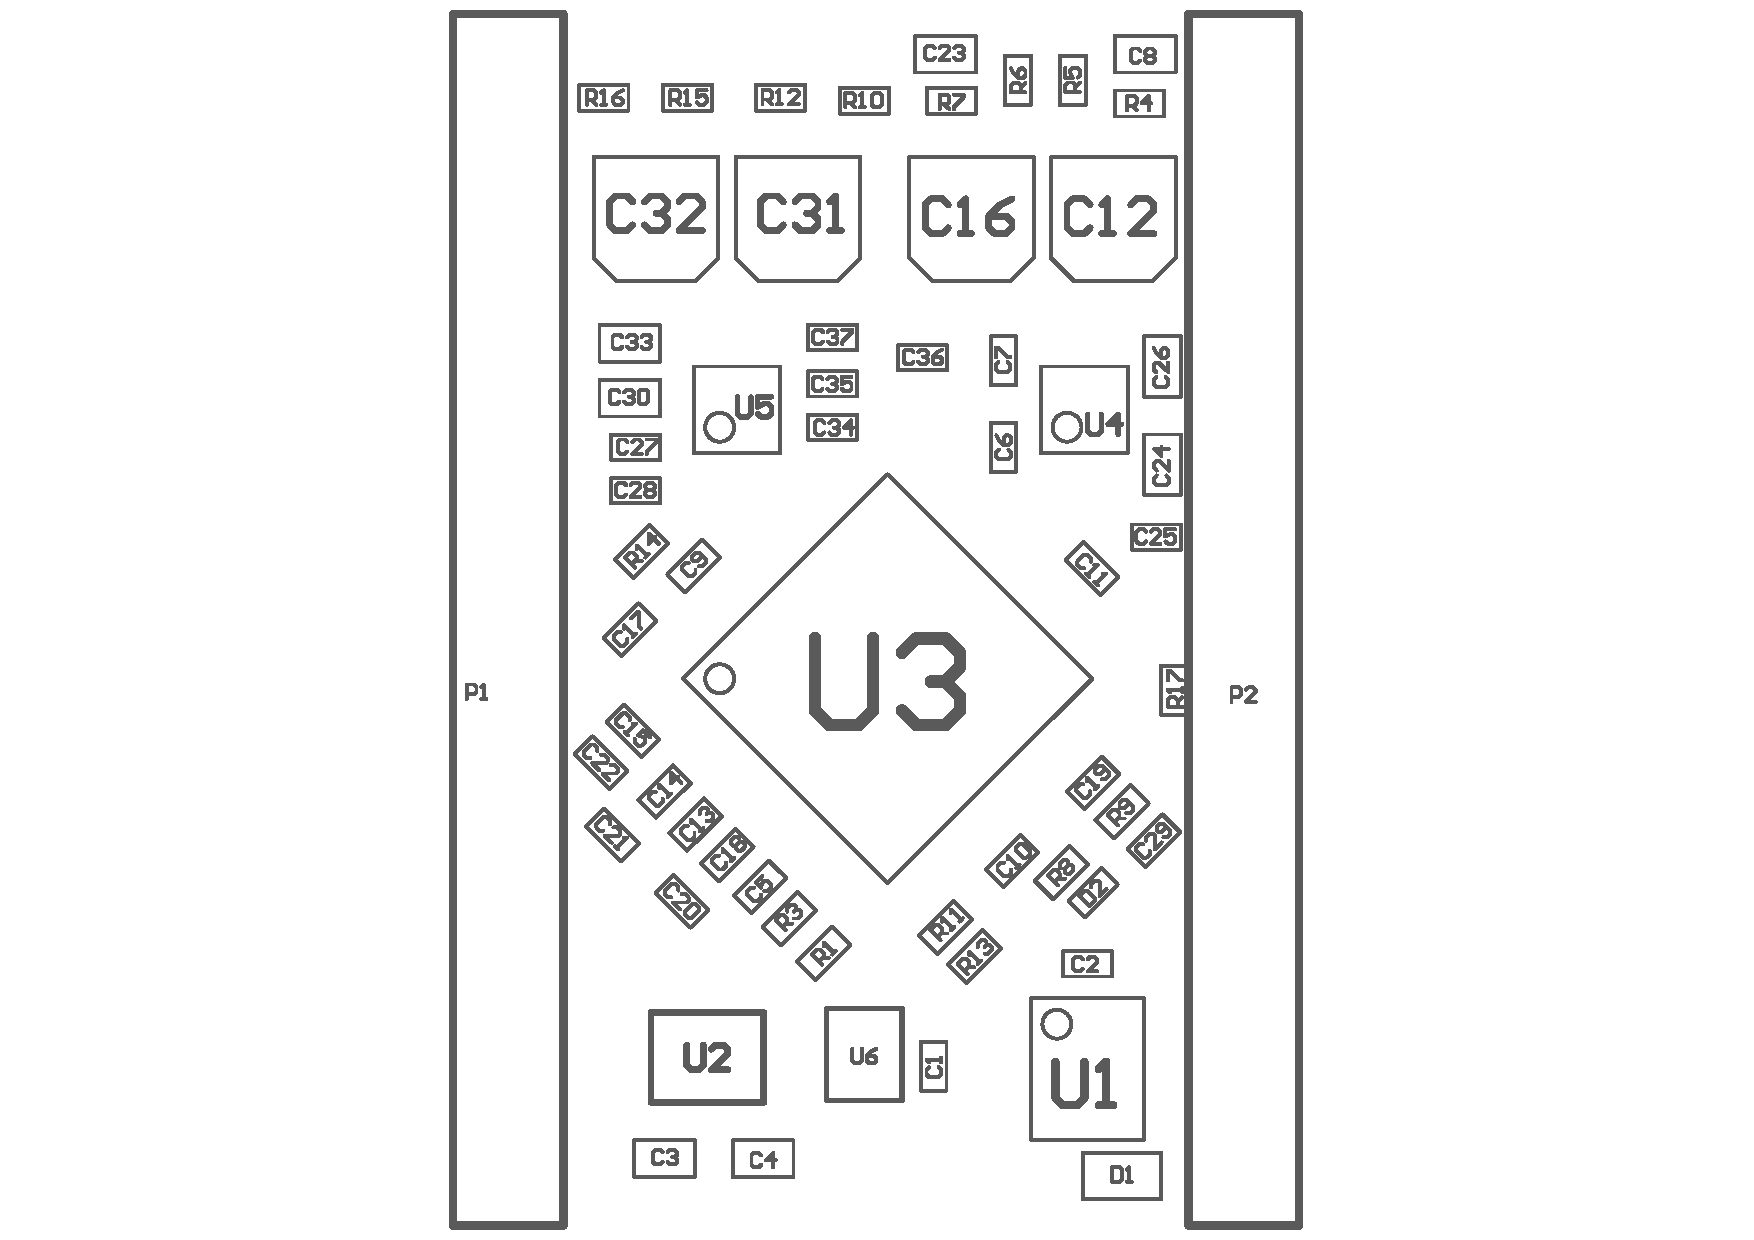
\includegraphics[scale = 1]{Assembly.pdf}
\vfill
\end{center}
\newpage

\section{Dimensions}
\vfill
\begin{center}
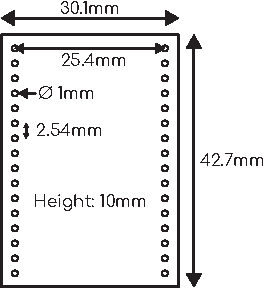
\includegraphics[scale = 3]{FXCore_Module_Dimensions.pdf}
\end{center}
\vfill
\newpage

\end{document}
